\documentclass[main.tex]{subfiles}
\begin{document}

For test generation, the ModelTestRelax(MTR,  Version: 3.5.16) framework \cite{mtr} was used with different parameters.

\subsection{Random Walk}
ThE Random Walk algorithm starts at an initial state and randomly selects a transition from the current state at each step. It stops when a specified condition is met, such as a percentage of states or transitions visited. While this method is useful for exploratory testing, it may generate longer test sequences than necessary for functional testing of complex systems. The algorithm supports FSMs and EFSMs, with an optional flag to include reset transitions in the coverage.

\subsubsection*{Execution and Parameters}
The algorithm is executed using the following parameters:
\begin{itemize}
    \item Coverage type: States or transitions.
    \item Coverage percentage: Desired percentage of coverage.
    \item Reset transitions: Optionally include reset transitions in coverage calculations.
\end{itemize}

\subsubsection*{Results}
For this analysis, \textit{Random Walk} was run with 100\% state and transition coverage and also with 75\% state and transition coverage as the stop condition. The last one was repeated five times to account for variability in sequence length and coverage.

\textbf{Results:} After running the Random walk(75\% transition coverage) 5 times, the following statistics can be made.
\begin{table}[H]
\centering
\begin{tabular}{|c|c|c|c|c|}
\hline
 & \textbf{Test Generation Time} & \textbf{Test Sequence Length} & \textbf{Reached coverage} \\ \hline
1 & 0.001434 s & 264 & 77.42\% \\ \hline
2 & 0.0009943 s & 72 & 77.42\% \\ \hline
3 & 0.0008907 s & 58 & 77.42\% \\ \hline
4 & 0.0010825 s & 75 & 77.42\% \\ \hline
5 & 0.0008158 s & 88 & 77.42\% \\ \hline
\textbf{Average} & \textbf{0.00104346
 s} & \textbf{111.4} & \textbf{77.42\%} \\ \hline
\end{tabular}
\caption{Summary of Random Walk Algorithm (5 Runs)}
\label{table:random_walk_summary}
\end{table}
Here we can see that there was one case (namely the first one) where it took much longer time and test sequence to reach the desired coverage or exceed it, which was 77.42\% all of the cases.  The outstanding long first run is not that surprising since it is a randomized algorithm, if it "chooses worng" multiple times, it will finish later.


\subsection{All-State}
The All-State algorithm generates a test sequence that ensures every state in a deterministic, strongly connected FSM is visited at least once. It uses the Nearest Neighbor heuristic to move towards the closest unvisited state in each step. Although reset transitions can be included, guard conditions in EFSMs are ignored. 

\textbf{Key Characteristics:}
\begin{itemize}
    \item Guarantees 100\% state coverage, but not transition coverage.
    \item Time complexity: $O(n^2)$, where $n$ is the number of states.
    \item Sequence length: $O(m)$, where $m$ is the number of transitions.
\end{itemize}

\subsubsection*{Execution and Parameters}
No additional parameters are required for FSMs, but the \texttt{--consider\_reset\_transitions} flag can be used for including reset transitions.
The following figure is an example run on the FSM model.
\begin{figure}[H]
    \centering
    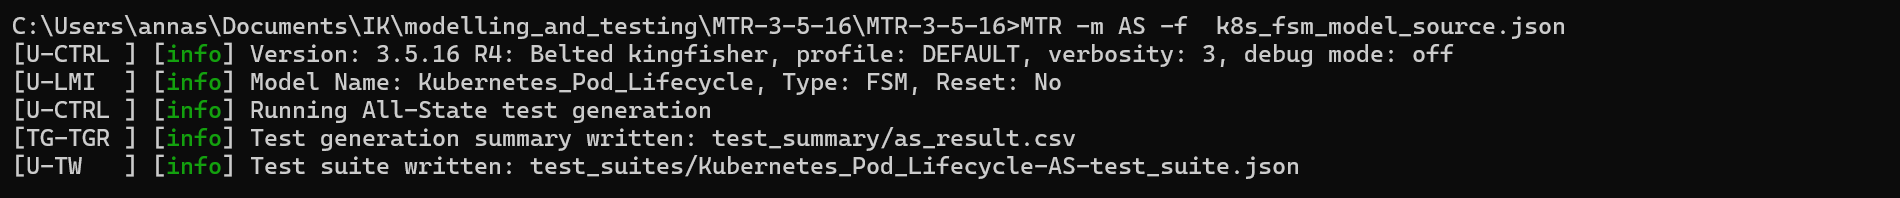
\includegraphics[width=\textwidth]{test_results/AS.png}
    \caption{All-state}
    \label{fig:all_state}
\end{figure}


\subsection{Transition Tour}
The Transition Tour algorithm produces a sequence covering every transition in a reduced, deterministic, strongly connected FSM, returning to the initial state afterward. It ensures 100\% state and transition coverage by solving the Directed Chinese Postman Problem, creating an Eulerian graph and finding an Euler tour. The algorithm has a time complexity of $O(n^3 + m)$ and sequence length $O(m)$. Reset transitions and Graphviz outputs are supported.

The following figure is an example run on the FSM model.
\begin{figure}[H]
    \centering
    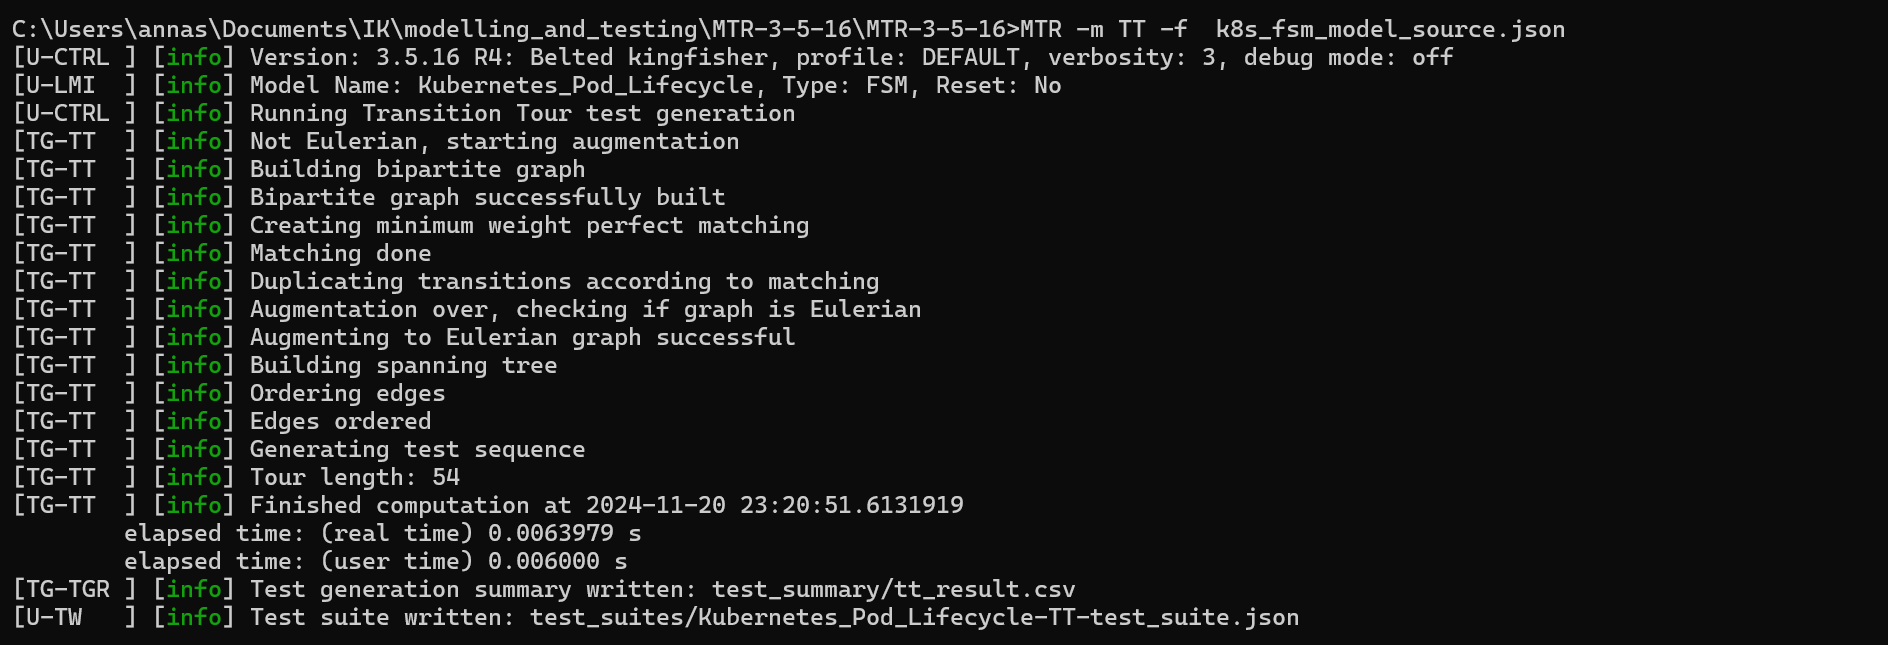
\includegraphics[width=\textwidth]{test_results/TT.png}
    \caption{All-state}
    \label{fig:all_state}
\end{figure}

\subsection{Directed Chinese Postman}
An extension of the Transition Tour, this algorithm considers transition costs too. It adjusts the test sequence by minimizing duplication costs while achieving the same coverage and complexity as Transition Tour. If transition costs are uniform, the sequences generated are identical to those of Transition Tour.
The use of this algorithm turned out to be useful when writing the adaptation code, where it became clear that some transitons like the clean up process or the image pulling take much longer time than others. So the previous FSM model was extended with costs and then the DCP could be run on it:

\begin{figure}[H]
    \centering
    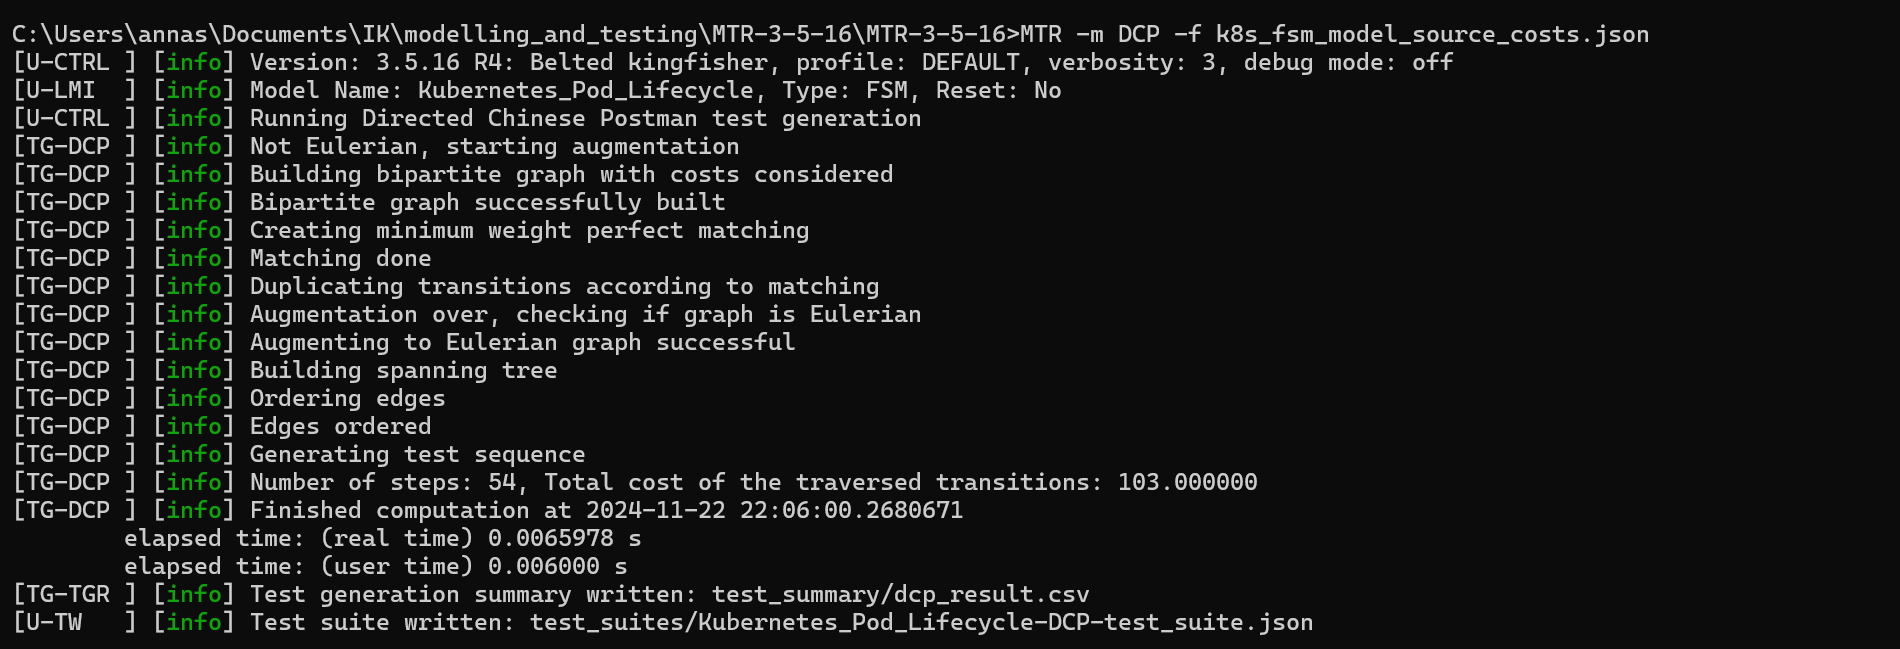
\includegraphics[width=\textwidth]{test_results/dcp.png}
    \caption{DCP}
    \label{fig:all_state}
\end{figure}

\subsection{All-Transition-State (ATS)}The ATS algorithm ensures all transitions and states of a reduced, deterministic FSM are covered based on two criteria: every transition must lead to all states, and there must be paths to all states excluding that transition (if feasible). The algorithm includes standard and iterative versions, trading off coverage and sequence length. The standard version has a complexity of $O(n^3 + m)$, while iterative versions increase complexity based on iteration limits.


\subsection{N-Switch Coverage}  
The N-Switch Coverage algorithm generates test sequences that cover all possible consecutive \(N+1\) transitions in the model, including loops. The parameter \(N\), set with the \texttt{--ns\_value} flag, determines the depth of coverage, allowing engineers to balance test sequence length and fault coverage. The algorithm iteratively selects uncovered transitions from an ordered list, augments sequences to cover partially completed paths, and stops when all transitions are fully covered. Additional tuning options, such as \texttt{--ns\_search\_depth}, enable optimization of test generation complexity versus sequence length. This method is well-suited for thorough testing of systems with complex state transitions, though it may require significant computational resources for large \(N\).

\begin{figure}[H]
    \centering
    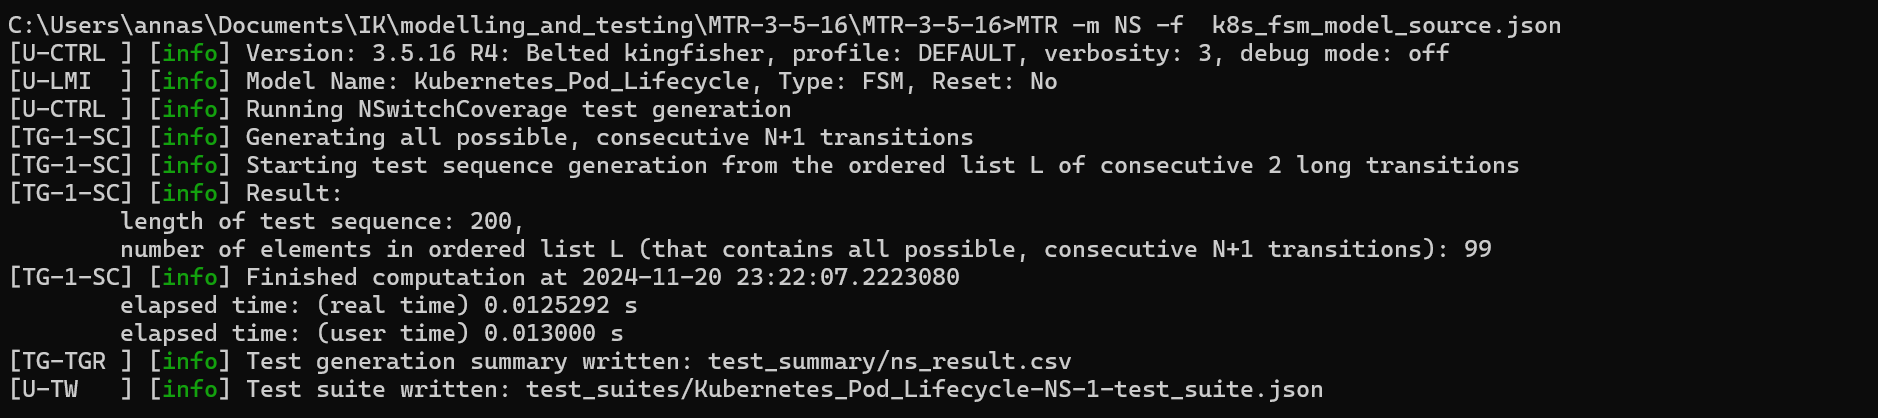
\includegraphics[width=\textwidth]{test_results/n-switch.png}
    \caption{All-state}
    \label{fig:all_state}
\end{figure}

\subsection{Comparison of Test Generation Algorithms}

Table~\ref{tab:algorithm_comparison} summarizes the performance of the selected algorithms based on the FSM model of Kubernetes pod lifecycle management.

\begin{table}[H]
\centering
\caption{Comparison of Test Generation Algorithms}
\label{tab:algorithm_comparison}
\begin{tabular}{|l|c|c|c|}
\hline
\textbf{Algorithm}     & \textbf{Test Sequence Length}     & \textbf{Elapsed Time}      & \textbf{Coverage} \\ \hline
Random Walk (100\% transition c.)     & 965     & 0.0052706 s    & 100\% transition coverage  \\ \hline
All-State     & 18     & 0,0001648 s    & 100\% state coverage \\ \hline
Transition Tour     & 54     & 0.0063979 s  & 100\% state- and transition coverage    \\ \hline
DCP     & 54     &  0.0065978 s  & 100\% state- and transition coverage    \\ \hline
All-Transition-State (standard)     & 193     & 0.0244396 s     & 100\% state- and transition coverage    \\ \hline
N-Switch Coverage (N=1)     & 200     & 0.0125292 s     & 100\% state- and transition coverage    \\ \hline
\end{tabular}
\end{table}

\subsection{Conclusions}
The Random Walk (100\% transition coverage) algorithm generated the longest test sequence, consisting of 965 steps, with a moderate elapsed time of 0.00527 seconds, emphasizing complete transition coverage but at the cost of producing lengthy sequences. In contrast, the All-State algorithm created the shortest test sequence of only 18 steps and was the fastest, with an execution time of 0.000165 seconds, as it focuses solely on state coverage, resulting in minimal generation. The Transition Tour algorithm generated a moderate sequence of 54 steps but took slightly longer, with an elapsed time of 0.00640 seconds, reflecting its method of traversing transitions optimally to ensure coverage. DCP had the same length of the generated test sequence, which was expected, the differences will be discovered when executing the test cases. The All-Transition-State (ATS) algorithm achieved comprehensive state and transition coverage, producing a sequence of 193 steps but with the highest elapsed time of 0.02444 seconds due to its detailed coverage requirements. Lastly, the N-Switch Coverage (N=1) algorithm provided a balance, generating a sequence of 200 steps with a reasonable elapsed time of 0.01253 seconds, focusing on transitions within a specified depth. These results demonstrate a clear trade-off between coverage, sequence length and execution time.


The generated test suites and result can be found in the github repository: \url{https://github.com/annasz11/kubernetes-mbt}.


\end{document}